\documentclass[border=6pt]{standalone}
\usepackage{fontspec,unicode-math}
\setmainfont{Noto Serif}
\setmathfont{STIXTwoMath-Regular.otf}
\usepackage{tikz}
\usetikzlibrary{arrows.meta,calc,patterns,decorations.markings,decorations.pathmorphing,decorations.pathreplacing}
\tikzset{lev/.style={line width=1.18pt,line cap=butt},
 fine/.style={line width=.55pt},light/.style={line width=.4pt},
 curve/.style={line width=1.18pt,line cap=round,line join=round},
 ax/.style={line width=.62pt,-{Latex[length=2.15mm,width=1.2mm]}},
 ray/.style={line width=.64pt,-{Latex[length=1.9mm,width=1.0mm]}},
 dim/.style={line width=.52pt,{Latex[length=1.65mm,width=.85mm]}-{Latex[length=1.65mm,width=.85mm]}},
 flow/.style={line width=.60pt,postaction={decorate},decoration={markings,mark=at position .62 with {\arrow{Latex[length=1.9mm,width=1.0mm]}}}},
 lab/.style={font=\fontsize{13}{16}\selectfont,inner sep=1.5pt},
 small/.style={font=\fontsize{11.2}{13.5}\selectfont,inner sep=1.2pt},
 panel/.style={font=\fontsize{13}{16}\selectfont\itshape,inner sep=1.5pt}}
\pagestyle{empty}
\begin{document}
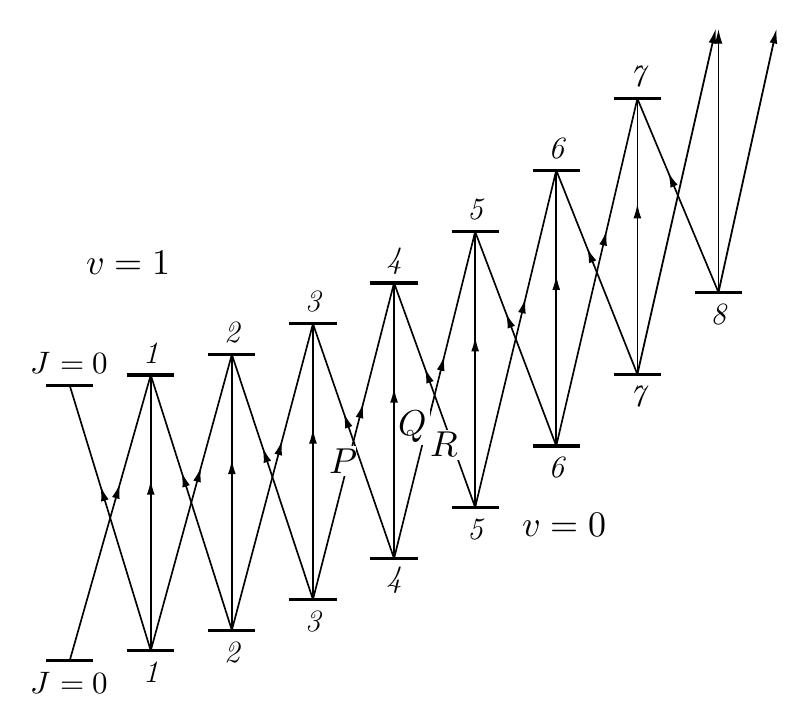
\begin{tikzpicture}[x=1cm,y=1cm,line join=round]
% Corrected E1 variant (original source drawing preserved in pre_corrector_figures/F15_11.tex).
\draw[lev] (-0.300000,0.000000)--(0.300000,0.000000);
\node[small] at (0.000000,-0.280000) {$J=0$};
\draw[lev] (0.730000,0.130000)--(1.330000,0.130000);
\node[small] at (1.030000,-0.150000) {$\textit{1}$};
\draw[lev] (1.760000,0.390000)--(2.360000,0.390000);
\node[small] at (2.060000,0.110000) {$\textit{2}$};
\draw[lev] (2.790000,0.780000)--(3.390000,0.780000);
\node[small] at (3.090000,0.500000) {$\textit{3}$};
\draw[lev] (3.820000,1.300000)--(4.420000,1.300000);
\node[small] at (4.120000,1.020000) {$\textit{4}$};
\draw[lev] (4.850000,1.950000)--(5.450000,1.950000);
\node[small] at (5.150000,1.670000) {$\textit{5}$};
\draw[lev] (5.880000,2.730000)--(6.480000,2.730000);
\node[small] at (6.180000,2.450000) {$\textit{6}$};
\draw[lev] (6.910000,3.640000)--(7.510000,3.640000);
\node[small] at (7.210000,3.360000) {$\textit{7}$};
\draw[lev] (7.940000,4.680000)--(8.540000,4.680000);
\node[small] at (8.240000,4.400000) {$\textit{8}$};
\draw[lev] (-0.300000,3.500000)--(0.300000,3.500000);
\node[small] at (0.000000,3.780000) {$J=0$};
\draw[lev] (0.730000,3.630000)--(1.330000,3.630000);
\node[small] at (1.030000,3.910000) {$\textit{1}$};
\draw[lev] (1.760000,3.890000)--(2.360000,3.890000);
\node[small] at (2.060000,4.170000) {$\textit{2}$};
\draw[lev] (2.790000,4.280000)--(3.390000,4.280000);
\node[small] at (3.090000,4.560000) {$\textit{3}$};
\draw[lev] (3.820000,4.800000)--(4.420000,4.800000);
\node[small] at (4.120000,5.080000) {$\textit{4}$};
\draw[lev] (4.850000,5.450000)--(5.450000,5.450000);
\node[small] at (5.150000,5.730000) {$\textit{5}$};
\draw[lev] (5.880000,6.230000)--(6.480000,6.230000);
\node[small] at (6.180000,6.510000) {$\textit{6}$};
\draw[lev] (6.910000,7.140000)--(7.510000,7.140000);
\node[small] at (7.210000,7.420000) {$\textit{7}$};
\node[lab] at (0.750000,5.050000) {$v=1$};
\node[lab] at (6.280000,1.720000) {$v=0$};
% OMITTED in corrected E1 schematic: forbidden J=0 to J=0, delta-J=0 is not allowed for J=0.

\draw[flow] (0.000000,0.000000)--(1.030000,3.630000);
\draw[flow] (1.030000,0.130000)--(0.000000,3.500000);
\draw[flow] (1.030000,0.130000)--(1.030000,3.630000);
\draw[flow] (1.030000,0.130000)--(2.060000,3.890000);
\draw[flow] (2.060000,0.390000)--(1.030000,3.630000);
\draw[flow] (2.060000,0.390000)--(2.060000,3.890000);
\draw[flow] (2.060000,0.390000)--(3.090000,4.280000);
\draw[flow] (3.090000,0.780000)--(2.060000,3.890000);
\draw[flow] (3.090000,0.780000)--(3.090000,4.280000);
\draw[flow] (3.090000,0.780000)--(4.120000,4.800000);
\draw[flow] (4.120000,1.300000)--(3.090000,4.280000);
\draw[flow] (4.120000,1.300000)--(4.120000,4.800000);
\draw[flow] (4.120000,1.300000)--(5.150000,5.450000);
\draw[flow] (5.150000,1.950000)--(4.120000,4.800000);
\draw[flow] (5.150000,1.950000)--(5.150000,5.450000);
\draw[flow] (5.150000,1.950000)--(6.180000,6.230000);
\draw[flow] (6.180000,2.730000)--(5.150000,5.450000);
\draw[flow] (6.180000,2.730000)--(6.180000,6.230000);
\draw[flow] (6.180000,2.730000)--(7.210000,7.140000);
\draw[flow] (7.210000,3.640000)--(6.180000,6.230000);
\draw[flow] (7.210000,3.640000)--(7.210000,7.140000);
\draw[ray] (7.210000,3.640000)--(8.205969,8.030000);
\draw[flow] (8.240000,4.680000)--(7.210000,7.140000);
\draw[ray] (8.240000,4.680000)--(8.240000,8.030000);
\draw[ray] (8.240000,4.680000)--(8.978865,8.030000);
\node[lab,fill=white,inner sep=1pt] at (3.448600,2.532400) {$P$};
\node[lab,fill=white,inner sep=1pt] at (4.360000,2.980000) {$Q$};
\node[lab,fill=white,inner sep=1pt] at (4.750200,2.741000) {$R$};

\end{tikzpicture}
\end{document}
